%intro
%	db=entity, store data structured manner, little redundancy, allow user access, controlled concurrent access
%	useful: efficent data access and storage, concurrent, user access rights
%	describe scenario
%Queries & results
%	Just dump query txt and csv file into doc, give BRIEF desc
%Description
%	ER Model
%		Start with own, show errors, show given one, explain how fix errors
%	Relation Scheme
%		Entity types, own table with attribs as columns, apply primary/compund key constraint
%		Compound attribs, move into tabel as sperate arribs
%		Convert Staff subtypes into own tables, with one-to-one relationship with Staff table
%		Add tables for many-to-many relationships, one col is id of one relation and the other is the id of the other
%		Add relationship attribs to the relations which needs them
%		Add forgien key contraints for all relationships, including the resursive ones
%		Issue adding staff data sue toi recusive relationship, removed relationaship will adding data, then readd
%Conclusion & Reflections
%	Understand relationship attribs, integral for optimal design, could be worked around but not good design, not much effort as table for relationship existed
%	Failed fully understand combining multiple queries, allows for better query design, more processing done by DBMS the better

\documentclass[12pt]{article}
\usepackage{listings}
\usepackage{graphicx}

\author{Stuart Reilly}
\date{\today}
\title{CS1Q - Information Management Report}

\begin{document}
\maketitle

\newpage
\tableofcontents

\newpage

\section{Introduction}
A database is an entity which stores data in a structured manner while minimising redunancy, allowing user access and controlled concurrent access.
Before databases became popular, data was stored in files.
This did not allow for concurrent access of the data as the operating system would restrict the number of user with access to each file.
Also, there was no way to link the data, which caused redunancy.
Finally, each program would have to implement some form structure to its data, which causes potential inconsitances between programs.
Databases solved these problems by allowing data to be linked through relationships and creating an abstraction between the physical layout of the data on disk and the program using it.
By providing the abstraction, any programs which use the data can access the data in the same way.
In order to allow for concurrent access of the data, a database management system will lie between programs and the database.
The database managment system will monitor and control who is trying to access the database, locking sections of the database while users use them.
This allows controlled concurrent access to the database, and allowing different user to be able to carry out a subset of the avalible database operations.
\\
\\
I was tasked to design and implement a database for the School of Computer Science which stores the details of students, courses, lecturer, assessments, tutorial groups and tutors.
It will store which student take which courses, the lecturers which teach each course and the assessments each student takes for their courses.
Also, which course has tutorial groups, which students are in each tutorial group and the tutor which leads each tutorial group.

\section{Queries And Results}
\subsection{Query 1}
\subsection{Query 2}
\subsection{Query 3}
\subsection{Query 4}
\subsection{Query 5}
\subsection{Query 6}

\section{Description}
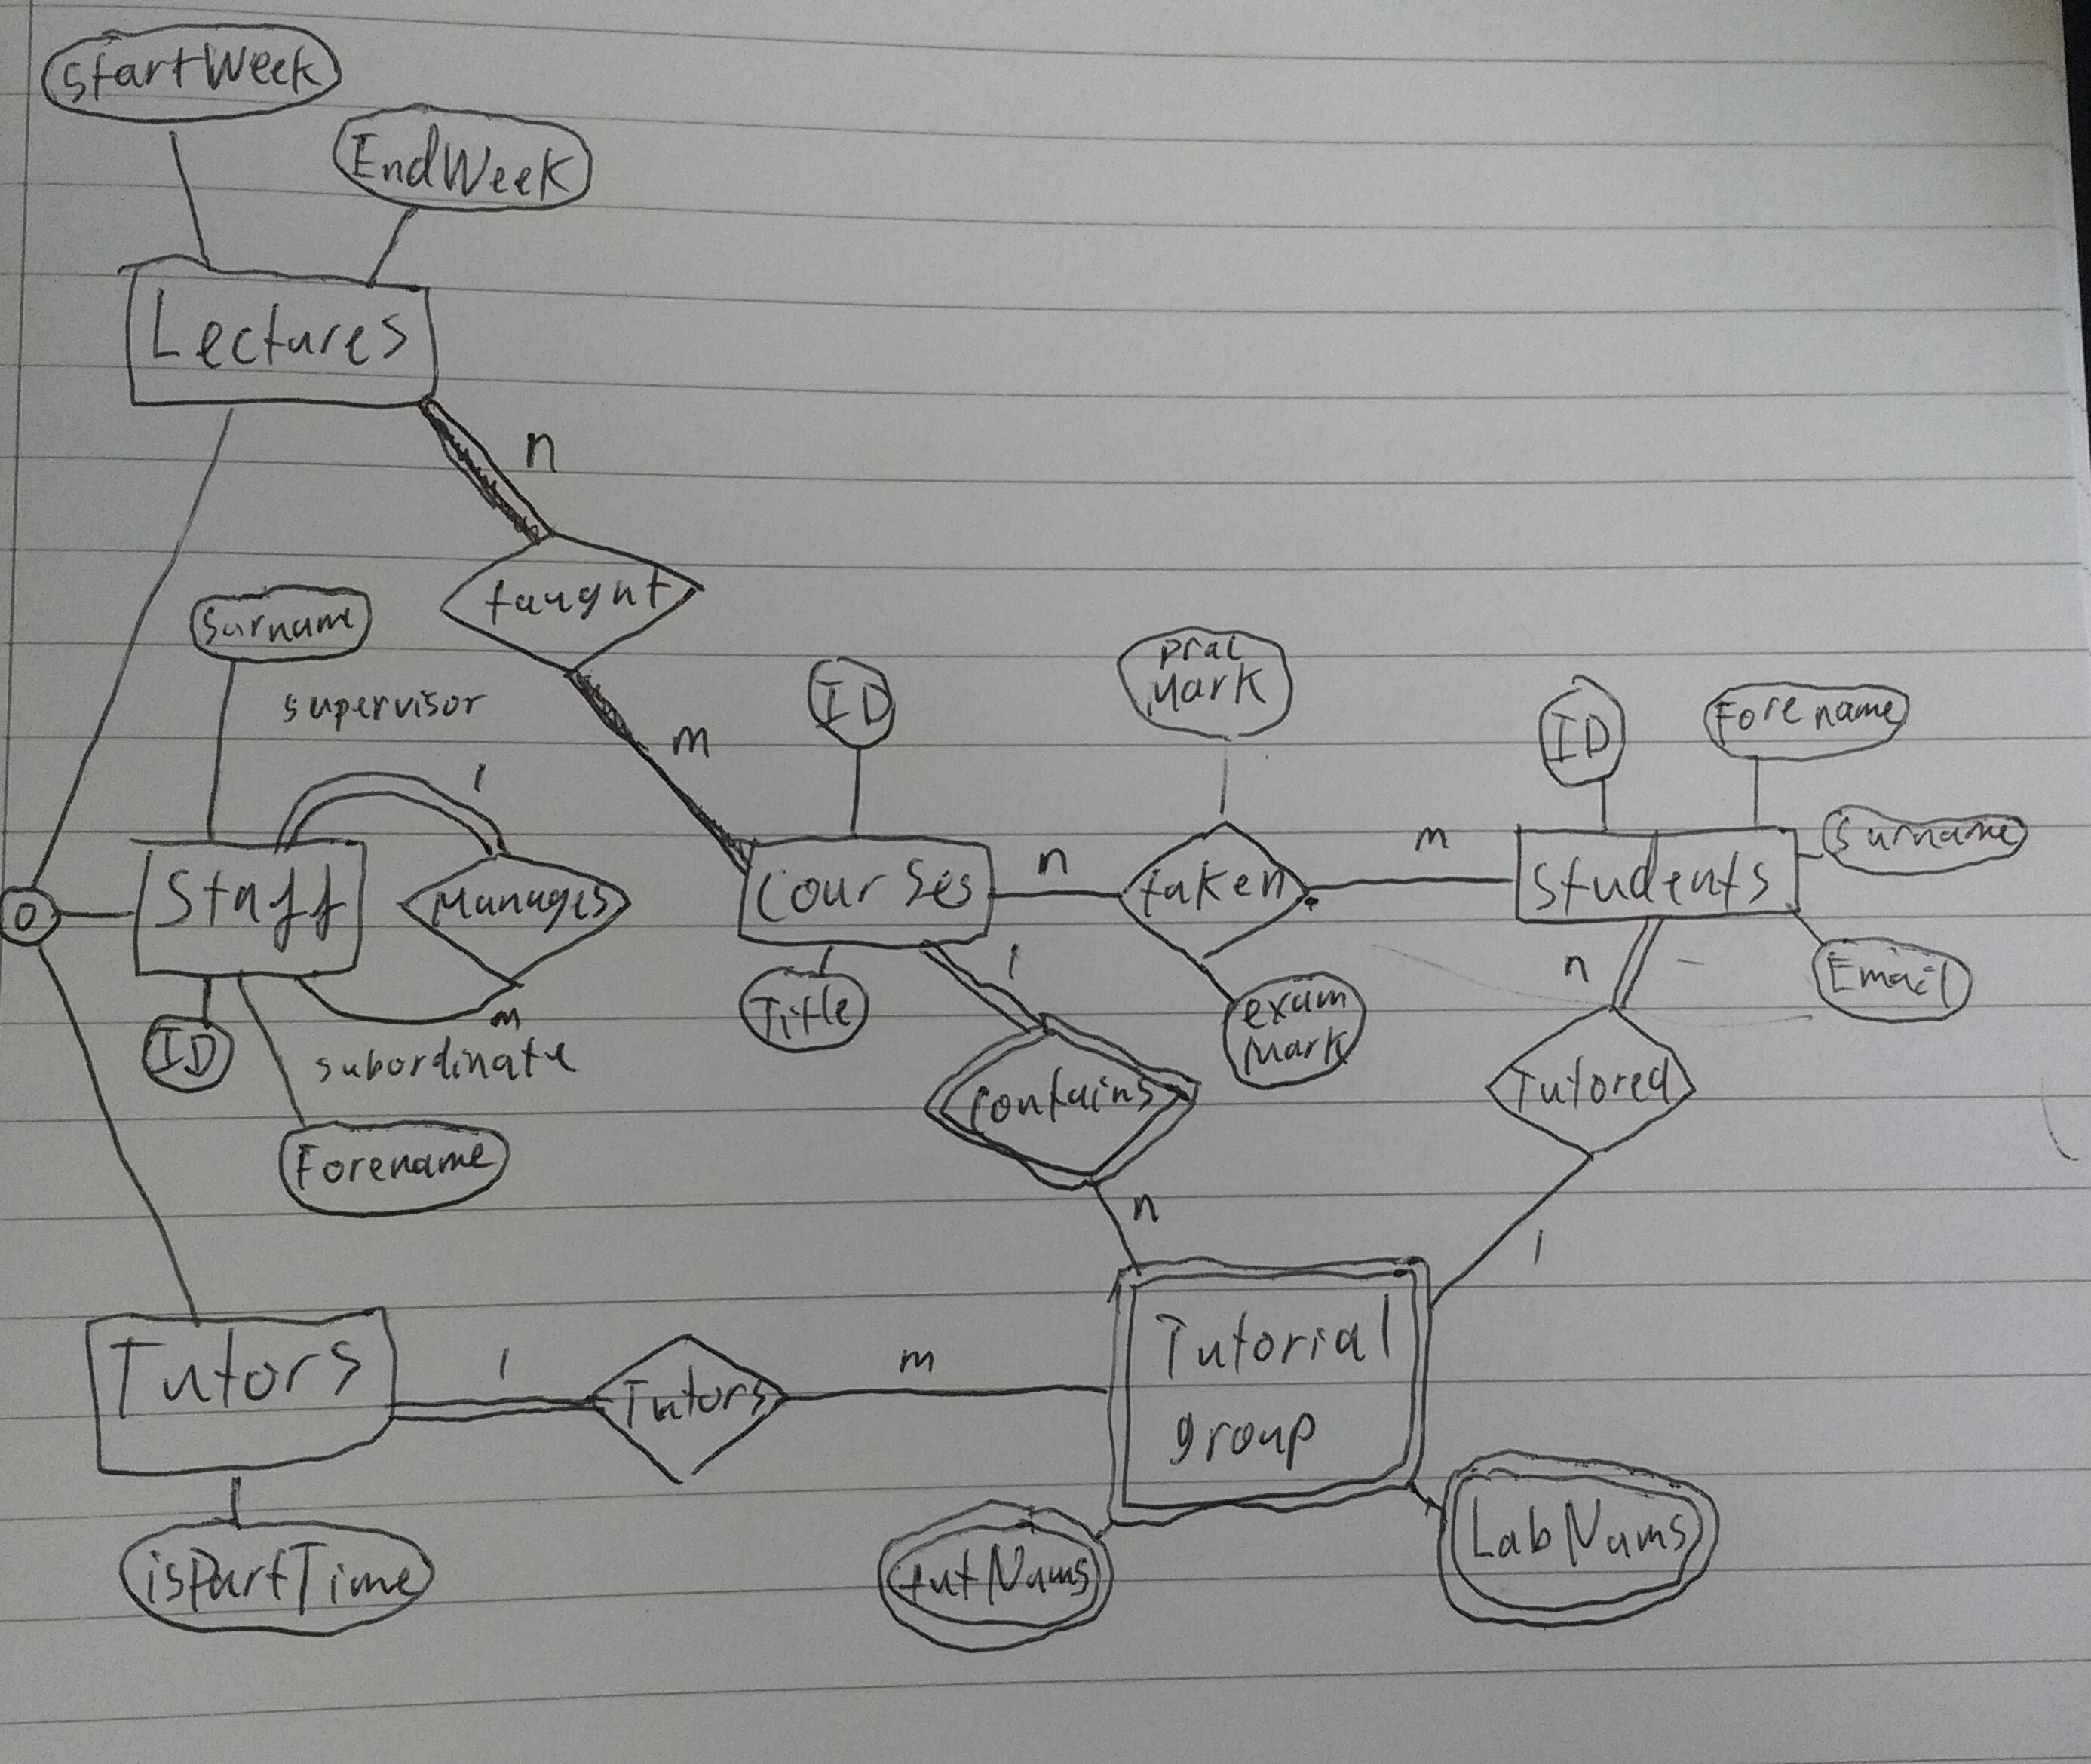
\includegraphics[width=\linewidth]{ER}
The above diagram is the initial enitity relationship diagram I produced from the given brief, which had a number of flaws in its design.
Firstly, the Staff entity type is missing its status attribute, which is required to determine the type of member of staff an entity is.
Next, the recursive relationship, to show which member of staff manages other member of staff, the supervisor side does not require total participation.
The issue has occured with both sides of trhe lecture-courses relationship the one side of the courses-tutorial group relationship and the many side of the students-tutorial group relationship.

\end{document}
